	
\chapter{Da sistemare }
\subsubsection{Derivation of I evolution and SIR differential equations presentation}
After having theoretically presented the model, it is now explained one method to derive the mathematical form of the infection compartment evolution. 
The set of differential equations that  describe the dynamic of infection is the following:
\begin{equation}
	\begin{cases}
		dS(t) / dt = -\beta S(t) I(t)\\
		dI(t) / dt = \beta S(t) I(t) - \gamma I(t)\\
		dR(t) / dt =  \gamma I(t)
	\end{cases}
\end{equation}
Here $X(t)$ is indicated as the population at time $t$ in the X compartment. Remember that the assumption of constant population size is also done, so $S(t)+I(t)+R(t) = N$ holds.

The number of infected, with an interval  $\Delta t$, that in a base case can coincide with one day, is given by the equation:
\begin{equation}
	I(t+\Delta t) = I(t) + [\beta S(t)I(t)/N - \gamma I(t)]\Delta t
\end{equation}

If the value of N is large, the variables can be considered as continuous, and imposing a time interval close to zero it becomes:

\begin{equation}
	\frac{d I(t)}{dt} = \lim_{\Delta t \rightarrow  0} \frac{I(t+\Delta t)-I(t)}{\Delta t} = \beta S(t) I(t)- \gamma I(t)
\end{equation}

Consider now the initial state of the system. At the beginning of the disease, considering that there are few infected, the majority of the population is in the susceptible groups, so $S(0) \approx N$. Furthermore, during the initial days of contagion diffusion, this quantity remains stable. Considering this approximation, we have 
\begin{equation}
	\frac{d I(t)}{dt} = (\beta S(0)-\gamma)I(t),
\end{equation} 
which gives now a differential equation with only a variable, $I(t)$, that has a well-known solution:

\begin{equation}
	I(t) = I(0) \exp ^{(\beta S(0)- \gamma)t}
	\label{eqn:sol_I}
\end{equation}



From the analytic solution of the infectious dynamic equation in \ref{eqn:sol_I}, we can see what happens at the beginning of an epidemic.  If the exponential argument has a positive sign it is observed an exponential increase in the number of infected. While, in the opposite case, infected people tend to zero. 
The value $\frac{ \beta}{\gamma} S(0) = 1$ is defined as the epidemic threshold. In the initial phase of the epidemic the relation $\frac{ \beta}{\gamma} S(0) = \frac{ \beta}{\gamma} N $  holds. 
This quantity, normalized, is called the basic reproductive rate, and indicated with the symbol $R_0$.

It measures the intensity of the contagion or the number of secondary infections a sick person can generate. Analysing the equation of susceptibles, with this model we see that it is always decreasing. In the SIR model, if the condition to start the epidemic is satisfied after an increase in the number of Infected, there is a point at which $\frac { \beta}{\gamma} S(0)$ becomes less than one. It is when this happens that the peak of the $I(t)$ curve is reached. Then, the disease begins its falling phase. It is the natural behavior of an epidemic.

\begin{figure}[h]
	\centering
	\subfloat[][\emph{}]
	{\includegraphics[width=0.48\linewidth]{0_introduction/images_introduction/sir_con_rt}} \quad
	\subfloat[][\emph{}]
	{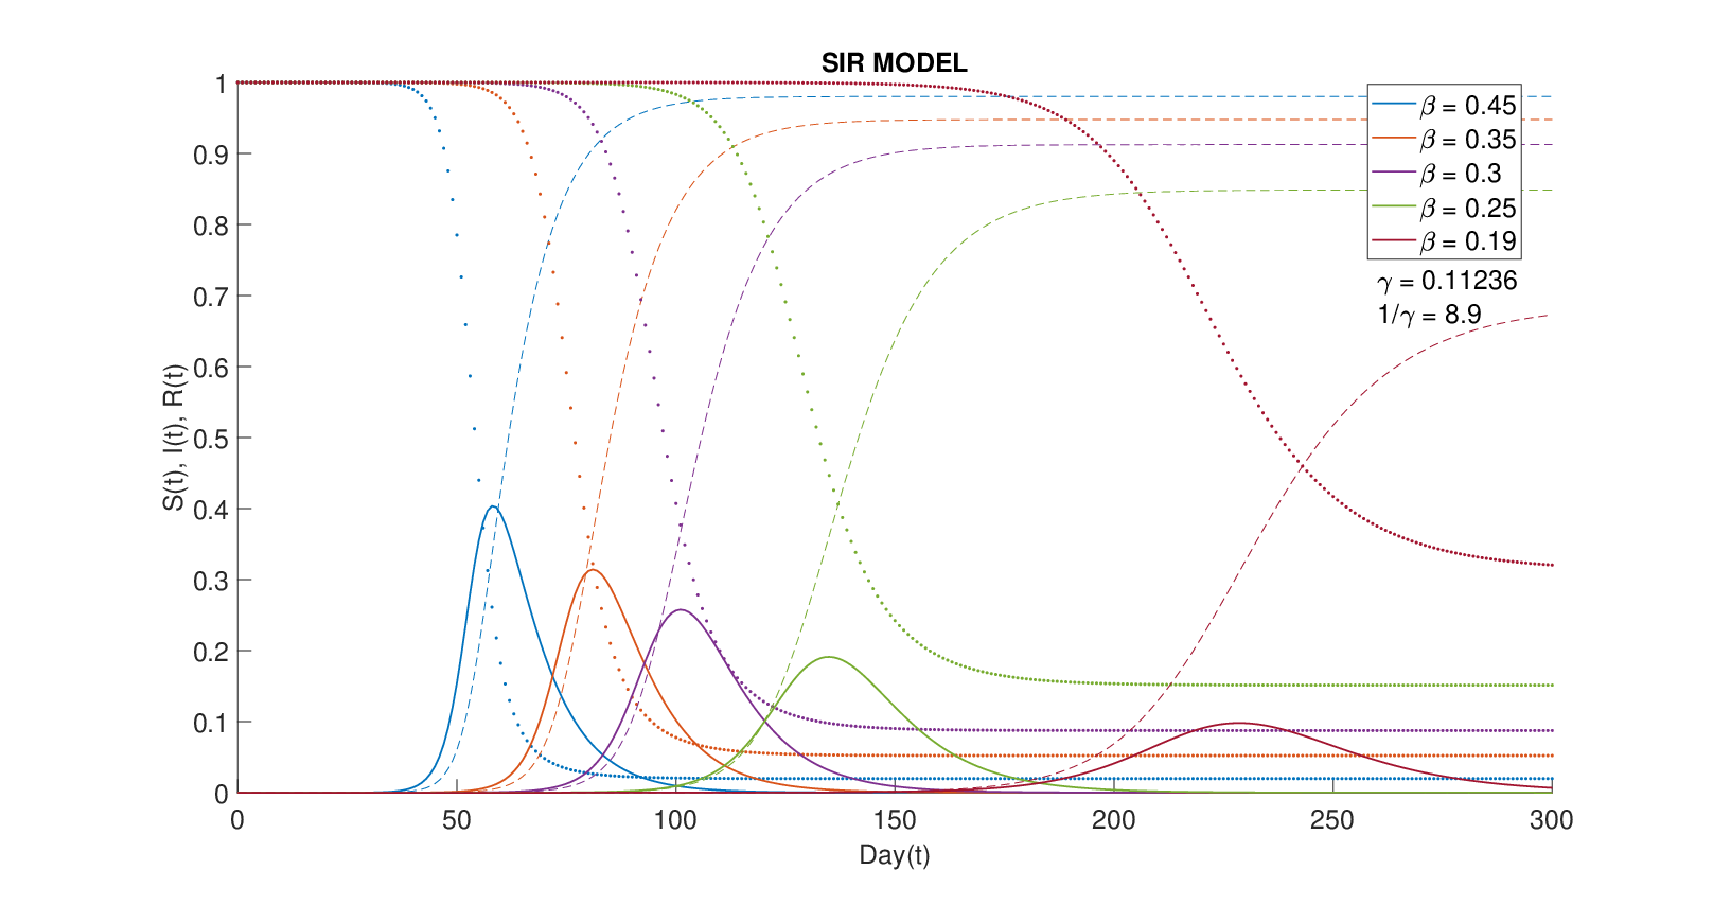
\includegraphics[width=0.48\linewidth]{0_introduction/images_introduction/sir_multipli_beta}} \\
	\caption[SIR dynamic example]{SIR system numerical solutions. Figure a) shows the evolution of compartments in the case of an epidemic. The violet dotted line represents the time-dependent $R_0(t)$. It can be seen that when this parameter is equal to $1$, the number of infected reaches its maximum value. In b) are presented different evolutions of the disease varying only the $\beta$ coefficient. The smaller its value the flattened and the more delayed the infectious curve is.}
	\label{fig:sir_example}
\end{figure}
Other two interesting quantities to consider when a new disease appears are the rate of increase of the infectious and the final size of remaining susceptible at the end of the epidemic. There is a large difference when a population suffers from an epidemic if this ends rapidly because a lot of people get sick or if this number can be controlled, and the infectious curve is flatter. A strategy to flatten the curve can reduce the contact between susceptibles, actuating social distancing or avoiding contact with infected, implementing quarantine measures. These are two simple examples of actions that reduce the value of $\beta$. Another countermeasure is represented by vaccination. Its immediate effect on the epidemic is to remove susceptibles people, so the disease can afflict only a small group and be quickly extinguished. 